\documentclass[../main.tex]{subfiles}

\begin{document}

\newpage

\section{QCD}%
\label{sec:qcd}

\subsection{Sterke interactie}%
\label{sub:sterke_interactie}

\begin{figure}[h]
    \centering
    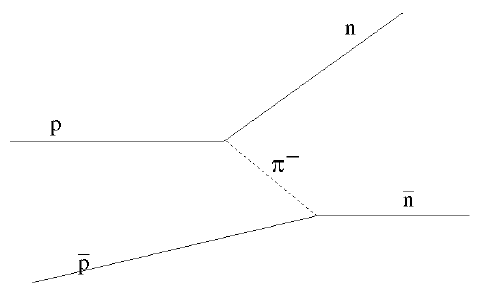
\includegraphics[width=0.6\linewidth]{QCD/ppnn.png}
    \caption{omvorming van protonen in neutronen}%
    \label{fig:ppnn}
\end{figure}

Historisch gezien is de sterke interactie ingevoerd om $p\overline p \rightarrow n\overline n$ te beschrijven. Hierbij werd gezegd dat deze nucleonen op vlak van kernkrachten gelijk zijn. en een sterk isospin doublet vormen.
\begin{equation}
    \begin{aligned}
        \label{eq:nucleon_doublet}
        \begin{pmatrix}
            p\\
            n
        \end{pmatrix}
        \text{: strek isospin}
    \end{aligned}
\end{equation}
Dit is een SU(2) groep en heeft 3 generatoren en uitwisselings deeltjes
\begin{equation}
    \begin{aligned}
        \label{eq:isospin_uitwisseling_deeltjes}
        \begin{pmatrix}
            \pi^+\\
            \pi^0\\
            \pi^-
        \end{pmatrix}
    \end{aligned}
\end{equation}
Dit werkt redelijk maar nu weten we natuurlijk dat dit niet correct is. Het grote probleem is dat deze uitwisselings deeltjes geen puntdeeltjes zijn. Wat tot technische problemen zal leiden. Normaal verwachten we ook dat bij deze sterke wisseling een vector boson het intermediair deeltje zou zijn met spin 1. De spin van de pionen is niet 1 maar 0 wat een groot probleem is. De reden waarom weten dat we een spin 1 deeltje nodig hebben als intermediair deeltje kunnen we halen uit het deterium dat we eerder besproken hebben. We hebben gezien dat er tussen het spin triplet en singlet een energie verschil zit en de spin weldegelijk zal uitmaken bij deze sterke interactie. We moeten dus gaan zoeken naar meer detail. Dit is dan uiteraard vervangen door het beeld dat we nu hebben met het proton en neutron bestaand uit quarks en deze die dan interageren met elkaar met behulp van gluonen.

\subsubsection{@ Quark level}%
\label{ssub:_quark_level}

Als we bij steeds hogere energie deze sterke interacties onderzoeken moeten we meer en meer rekening beginnen houden met de individuele bijdrages van de quarks. Bij deze hogere energieën kwam er nog een ander probleem naar boven dat kon gezien worden aan de hand van $\Delta^{++}=\left|u^\uparrow u^\uparrow u^\uparrow\right>$. We zien dat deze golffunctie volledig symmetrisch is.
\begin{itemize}
    \item Spaciaal: $l=0$
    \item Flavour: allemaal $u$ quarks
    \item Spin: zijn allemaal naar omhoog gericht
\end{itemize}
Wat tot dan totaal niet kon volgens Fermi. Om dit op te lossen wordt een nieuw kwantumgetal toegevoegd in de $SU(3)$ groep, kleur. Dit is het ontstaan van QCD. We zorgen dat de golffunctie van de kleur volledig antisymmetrisch is. De 3 nieuwe ladingen voor de kleur zijn
\begin{equation}
    \begin{aligned}
        \label{eq:kleur_lading}
        \begin{pmatrix}
            r\\
            g\\
            b
        \end{pmatrix}
    \end{aligned}
\end{equation}
Omdat we $SU(3)$ hebben  hebben we 8 generatoren wat neerkomt op 8 uitwisseling deeltjes.

\subsection{Symmetrie van de sterke wisselwerking}%
\label{sub:symmetrie_van_de_sterke_wisselwerking}

Het bewijzen dat er juist 3 kleur lading zijn gebeurd als volgt. We kijken naar de verhouding van de werkzame doorsnedes van $e^+e^-$ verval naar hadronen en muonen.
\begin{equation}
    \begin{aligned}
        \label{eq:experiment_sterke_sym}
        R(\sqrt{s}) &= \frac{\sigma(e^+e^- \rightarrow \text{hadrons})}{\sigma(e^+e^- \rightarrow \mu^+\mu^-)}\\
                    &= \frac{\sum_c\sum_q \int \left|
                        \feynmandiagram[inline=(a), horizontal=a to b]{
                        a -- [photon, edge label=\(\gamma\)] b,
                        i1 [particle=\(e^-\)] -- [fermion] a,
                        a -- [fermion] i2 [particle=\(e^+\)],
                        f1 [particle=\(q'\)] -- [fermion] b,
                        b -- [fermion] f2 [particle=\(q\)],
                    };
                    \right|^2}{\int \left|
                    \feynmandiagram[inline=(a), horizontal=a to b]{
                        a -- [photon, edge label=\(\gamma\)] b,
                        i1 [particle=\(e^-\)] -- [fermion] a,
                        a -- [fermion] i2 [particle=\(e^+\)],
                        f1 [particle=\(\mu^+\)] -- [fermion] b,
                        b -- [fermion] f2 [particle=\(\mu^-\)],
                    };
                    \right|^2}\\
                    &= N_c\sum_q Q_q^2
    \end{aligned}
\end{equation}
Het enige verschil tussen de 2 diagrammen naast de massa van de deeltjes is het ladingsverschil tussen de uitgaande deeltjes. We kunnen dus het aantal kleuren letterlijk waarnemen.

\begin{figure}[h]
    \centering
    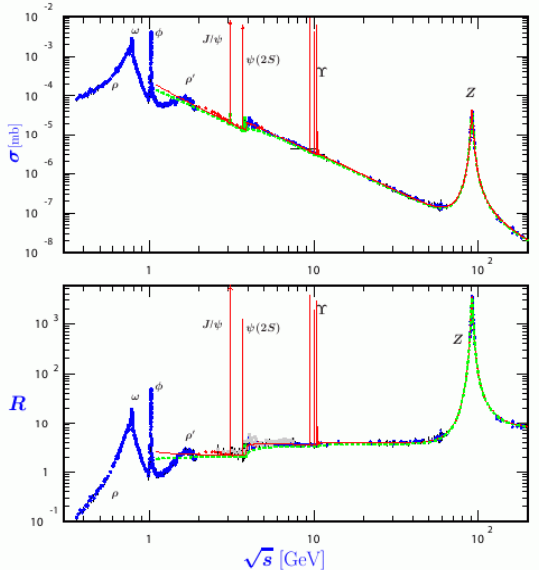
\includegraphics[width=0.8\linewidth]{QCD/ee_scattering.png}
    \caption{De resultaten van verschillende $e^+e^-$ verstrooiingen}%
    \label{fig:ee_scattering}
\end{figure}

Indien het foton maar juist genoeg energie heeft om een specifiek quark-antiquark paar aan te maken zullen deze niet van elkaar weg bewegen en krijgen we een resonanties die in figuur \ref{fig:ee_scattering} aan de hand van pieken waargenomen kunnen worden. Als je kijkt naar R is de stap achter $\psi$ piek. Het verschil tussen de 2 stappen geeft ons nu juist de lading van de $c$ quark. Omdat dit in stappen gaat is ook aangetoond dat de quarks elementaire deeltjes zijn. Anders zouden we niet die vlaktes zien. De groene curve is het equivalent van vergelijking (\ref{eq:experiment_sterke_sym}). De rode curve is iets ingewikkelder. Hierbij zijn de radiatieve correcties van gluonen ook in acht genomen. De nieuwe vergelijking voor $R$ gaat als volgt
\begin{equation}
    \begin{aligned}
        \label{eq:experiment_sterke_sym_extended}
        R(\sqrt{s}) = N_c\sum_q Q_q^2 (1+\frac{\alpha_s}{\pi})
    \end{aligned}
\end{equation}
Zo is het mogelijk om de sterke koppelingsconstante in functie van de energie uit te zetten. Als $\sqrt{s}\geq 2m_\tau$ dan is het ook mogelijk om $\tau$ te produceren. Deze kunnen vervallen in hadronen zelf en zal nog een extra correctie aan $R$ moeten toegevoegd worden.

\subsection{Kleur}%
\label{sub:kleur}

Met het invoeren van de kleuren is het probleem van $\Delta^{++}$ nu ook opgelost. De golffunctie hiervan kan nu zuiver antisymmetrisch gemaakt worden.
\begin{equation}
    \begin{aligned}
        \label{eq:golffunctie_baryon}
        \psi_{kleur}(B) &= \frac{1}{\sqrt{6}} [\left|rgb-rbg+brg-bgr+gbr-grb\right>]\\
                        &= \frac{1}{\sqrt{6}} \sum_{ijk} \epsilon^{ijk}c_ic_jc_k
    \end{aligned}
\end{equation}
Het singlet in kleur ruimte zal van een $3\otimes 3\otimes 3 = 1\oplus 8\oplus 8\oplus 10$ wat een singlet, 2 octetten en dictet zijn. Zo krijgen we uiteindelijk voor de kleur golffuncties van de (anti)baryonen en mesonen
\begin{equation}
    \begin{aligned}
        \label{eq:kleur_golffunctie}
        \psi_{kleur}(B) &= \frac{1}{\sqrt{6}} \sum_{ijk} \epsilon^{ijk}c_ic_jc_k\\
        \psi_{kleur}(\overline B) &= \frac{1}{\sqrt{6}} \sum_{ijk} \epsilon^{ijk}\overline c_i \overline c_j\overline c_k\\
        \psi_{kleur}(M) &= \frac{1}{\sqrt{3}} \left|r\overline r + b\overline b + g\overline g \right>
    \end{aligned}
\end{equation}
In de mesonen zien we dat we een volledig symmetrische kleur golffunctie hebben en wordt het anti symmetrisch zijn door andere golffuncties bepaalt.

\subsection{Gluonen}%
\label{sub:gluonen}

Omdat de sterke interactie een $SU(3)$ groep is hebben we 8 uitwisselings deeltjes $g_i$, de gluonen. Omdat $SU(3)$ niet Abels is kunnen deze deeltjes aan zelf interacties doen. Ze dragen dus hun eigen kleur en antikleur. Wat ervoor zorgt dat deze sterke interactie enkel werkt over korte afstanden. Je zou dus kunnen denken voor een meson dat $3\times 3 = 9$ maar dit is niet correct. De correcte rekening is $3\otimes 3 = 1 \oplus 8$. Het singlet heeft hier geen kleur en doet dus niet aan zelf interacties.

\subsection{Jets}%
\label{sub:jets}

De toestand van ons verstaan wat Jets nu precies doen is gecompliceerd. Nemen we de volgende interactie\\
\begin{center}
\feynmandiagram[inline=(a), horizontal=a to b]{
    a -- [photon, edge label=\(\gamma\)] b,
    i1 [particle=\(e^-\)] -- [fermion] a,
    a -- [fermion] i2 [particle=\(e^+\)],
    f1 [particle=\(\overline q\)] -- [fermion] b,
    b -- [fermion] f2 [particle=\(q\)],
};
\end{center}
Het overschot aan energie dat niet is gebruikt voor het maken van het quark-antiquark paar wordt gebruikt om de 2 quarks van elkaar weg te sturen. Dit uit elkaar gaan van de quarks zorgt ervoor dat ze gluonen zullen uitsturen die dan later combineren tot hadronen. Deze gekleurde intermediaire toestanden moeten op een of andere manier met elkaar spreken om als uiteindelijke toestanden niet gekleurde hadronen te bekomen. In dit hadronisatie process gaat veel informatie verloren. Om de originele partonen terug te bekomen moeten we aan Jet algoritmes doen. Dit is een iteratieve procedure die de volgende stappen herhaalt tot een bepaalt criterium is behaald.
\begin{enumerate}
    \item maak lijst van gedetecteerde objecten
    \item je plaatst de meest waarschijnlijke paren samen
    \item bereken de afstand tussen de 2
    \item degene met de kleinste afstand tussen elkaar worden gecombineerd
    \item ga door tot nog maar 1 paar over is of een voorwaarde is bereikt
\end{enumerate}
De afstandsschalen tussen deze deeltjes kunnen als volgt berekent worden
\begin{equation}
    \begin{aligned}
        \label{eq:jet_alg_afstand}
        \delta_{ij} = \sqrt{p_i^2+p_j^2} = m_{invariant}\\
        \delta_{ij} = \frac{2\text{min}(E_i^2,E_j^2)(1-\cos\theta_{ij})}{E_{visible}} 
    \end{aligned}
\end{equation}
Je kan deze impulsen ook samenstellen wat we de ``combinatie schema''.
\begin{equation}
    \begin{aligned}
        \label{eq:comb_scheme}
        p=p_i+p_j\\
        E=E_i+E_j
    \end{aligned}
\end{equation}
Een mogelijk criterium is het aantal jets dat er in een systeem worden waargenomen. Waarbij de mogelijkheid op het aantal jets kan weergegeven als volgt.\\
$n$-jets rates:
\begin{itemize}
    \item 2 jets: $\propto \alpha_s^0 = 1$
    \item 3 jets: $\propto \alpha_s^1$
    \item 4 jets: $\propto \alpha_s^2$
    \item ...
\end{itemize}
\end{document}
